% PlanArena technical supplement. Filled from results/ and from the code's own settings by planarena/paper.py:
%   python -I -m planarena.paper      (writes supplement.tex and, with tectonic, supplement.pdf). Do not edit supplement.tex.
\documentclass[10pt]{article}
\usepackage[margin=0.8in]{geometry}
\usepackage{fontspec}
\setmainfont{texgyretermes}[Extension=.otf, UprightFont=*-regular, BoldFont=*-bold,
  ItalicFont=*-italic, BoldItalicFont=*-bolditalic]
\usepackage{microtype}
\usepackage{booktabs}
\usepackage{graphicx}
\usepackage{amsmath}
\usepackage{placeins}
\usepackage[numbers,sort&compress]{natbib}
\usepackage[hidelinks]{hyperref}
\usepackage{caption}
\captionsetup{font=footnotesize,labelfont=bf,skip=3pt}
\usepackage{enumitem}
\setlist{nosep,leftmargin=*}
\usepackage[compact]{titlesec}
\titlespacing*{\section}{0pt}{8pt}{3pt}
\titlespacing*{\subsection}{0pt}{6pt}{2pt}
\titlespacing*{\paragraph}{0pt}{3pt}{0.6em}
\setlength{\parskip}{0.15em}
\setlength{\emergencystretch}{1.5em}
\graphicspath{{../docs/figures/}}
\renewcommand{\thetable}{S\arabic{table}}
\renewcommand{\thefigure}{S\arabic{figure}}
\renewcommand{\thesection}{S\arabic{section}}
\renewcommand{\theequation}{S\arabic{equation}}

\title{\vspace{-2em}\large\textbf{PlanArena: technical supplement}\\[0.2em]
\normalsize Model specification, test protocols and additional results}
\author{\normalsize Parya Payami\\ \footnotesize Department of Architecture, University of Wisconsin--Milwaukee}
\date{\footnotesize Draft, \today}

\begin{document}
\maketitle
\vspace{-1.5em}

\noindent This supplement specifies every model in the paper and the protocol of every test, so that each result can
be reproduced from the code and the public data. Settings marked $\dagger$ are read from the code when this document is
built. Section numbers refer to the paper unless prefixed with S.

\section{Types of evidence}\label{s:evidence}

The paper uses four kinds of evidence, which support different claims (Table~\ref{tab:s-evidence}).
\begin{itemize}
\item \textbf{Empirical predictive validation}: a prediction made with information available before an outcome,
compared with that outcome, on observations not used to build or select the model.
\item \textbf{Accounting check}: the model reproduces recorded quantities it was built from or calibrated to (for
example the baseline twin against assessor records). It shows the bookkeeping is right, not that predictions are.
\item \textbf{Algorithmic verification}: a search or rule is checked against a known answer (exhaustive enumeration,
exact re-scoring), independent of whether its objective is right.
\item \textbf{Illustrative simulation}: outputs that follow from stated assumptions (stakeholder utilities, seats) and
show how a decision depends on them. They have no observed counterpart.
\end{itemize}

\begin{table}[t]
\centering
\small
\setlength{\tabcolsep}{4pt}
\caption{Claims, the evidence behind them, and its type.}
\label{tab:s-evidence}
\begin{tabular}{llll}
\toprule
Component & Claim & Evidence & Test \\
\midrule
Existing conditions & records reproduced & accounting check & twin vs assessor, LL84, LEHD \\
Planning calculations & reviews' projections reproduced & accounting check & two environmental reviews \\
Impact engine & effects of observed change & empirical, held out & selection / evaluation folds \\
Job change & effect on jobs by block & empirical, held out (no skill) & LEHD 2015--2023 \\
Access, mix, green cover & effects of change & not validated & no after-change data \\
Redevelopment model & where change happens & empirical, out of time & rolling origins; seven cities \\
Calibration & how often change happens & empirical, out of time & reliability, O/E, Brier skill \\
Zoning and plan layers & added predictive value & empirical, out of time & block ablation, conservative variant \\
Housing projections & homes built & empirical, out of time & districts; three rezonings \\
Optimizer & best plan found & algorithmic verification & exhaustive search; benchmark \\
NSGA-III explorer & trade-off front & algorithmic verification & exhaustive enumeration of blocks \\
Realism layers & plausible recommendations & empirical, out of time & 2020 plans vs 2025 outcomes \\
Decision module & how a choice depends on its rule & illustrative simulation & assumed utilities and seats \\
\bottomrule
\end{tabular}
\end{table}

\section{Data timing and leakage audit}\label{s:leakage}

\paragraph{Feature timestamps.} Table~\ref{tab:s-timing} lists the source and date of every feature family for each
panel. In Manhattan every feature comes from the MapPLUTO release of the decision year $t_0$. In the cross-city panels,
zoning and plan layers are current layers in some cities; lots whose zoning or plan dates from $t_0$ or later are
flagged where the layer carries dates, and the conservative variant drops them. Dallas's zoning and plan are undated
current layers (the plan was adopted in 2024, after its $t_0$ of 2022), so its zoning and plan results may contain
post-decision information and are not unbiased estimates of what those layers add.

\begin{table}[t]
\centering
\footnotesize
\setlength{\tabcolsep}{4pt}
\caption{Source and date of each feature family against the decision year $t_0$. Context features (neighbour composition, recent construction within 400 m) come from the same record as existing conditions.}
\label{tab:s-timing}
\begin{tabular}{p{0.17\linewidth}p{0.22\linewidth}p{0.17\linewidth}p{0.17\linewidth}p{0.17\linewidth}}
\toprule
Panel & Existing conditions & Zoning & Plan & Measured after $t_0$ \\
\midrule
Manhattan (rolling origins, 2015-2025) & MapPLUTO release of year t0: use, lot and floor area, floors, year built, units, assessed land and total value & same release: zoning district, maximum FARs, overlays, landmark and historic status & none (no citywide adopted land-use plan) & none \\
Los Angeles & SCAG 2020 land use; assessor roll of t0 & SCAG 2019 compilation & SCAG 2019 General Plan compilation & none \\
Dallas & DCAD codes of t0 & current layer (undated) & forwardDallas! 2.0, adopted 2024 (after t0 = 2022) & zoning and plan may include changes after t0; no dates to remove them \\
Phoenix & MAG vintage of t0; assessor & current layer; zoning cases dated t0 or later flagged & General Plan 2015 as amended; polygons added after t0 flagged & flagged lots removed in the conservative variant \\
San Diego & SANDAG vintage of t0 & current layer; implemented on or after t0 flagged & General and community plans (undated) & zoning flags removed in the conservative variant; plan undated \\
New York City & MapPLUTO of t0 & MapPLUTO of t0 & none & none \\
Milwaukee & MPROP of t0 & MPROP of t0 & none (PDF only) & none \\
Chicago & CMAP inventory before t0; Cook County Assessor of t0 & current layer; districts created on or after t0 flagged & none & flagged lots removed in the conservative variant \\
\bottomrule
\end{tabular}
\end{table}

\paragraph{Following lots over time.} Each $t_0$ lot is followed to the $t_1$ lot that contains its representative
point. When several $t_0$ lots fall in one $t_1$ lot (a merger), their $t_0$ floor area is summed before growth is
measured, and each of them takes the merged lot's outcome. When one $t_0$ lot contains several $t_1$ lots (a split),
growth is measured on the piece that contains the $t_0$ point. Table~\ref{tab:s-identity} counts both. Lots with no
$t_1$ lot are left out.

\begin{table}[t]
\centering
\footnotesize
\setlength{\tabcolsep}{4pt}
\caption{Following Manhattan lots over time, and labels removed by the new-building rule.}
\label{tab:s-identity}
\begin{tabular}{lrrrrrrr}
\toprule
Pair & $t_0$ lots & No $t_1$ lot & Mergers & Lots merged & Splits & Developed & Removed \\
\midrule
2015--2016 & 42{,}786 & 0 & 92 & 239 & 24 & 913 & 1 \\
2015--2020 & 42{,}786 & 1 & 307 & 872 & 55 & 1{,}814 & 1 \\
2019--2020 & 42{,}441 & 1 & 60 & 182 & 10 & 313 & 0 \\
2020--2021 & 42{,}327 & 0 & 4 & 11 & 2 & 14 & 51 \\
2020--2025 & 42{,}327 & 1 & 153 & 472 & 43 & 520 & 50 \\
2024--2025 & 42{,}134 & 0 & 38 & 115 & 14 & 126 & 0 \\
\bottomrule
\end{tabular}
\end{table}

\paragraph{A label error found and corrected.} A building counts as new in $(t_0, t_1]$ only if it is not already on
the $t_0$ record with a year built of $t_0$ or later. The December 2020 MapPLUTO release (20v8) already lists
50 buildings completed in 2020; without this rule they were counted as developed in every pair starting
in 2020 (78\% of the 2020--2021 positives and 9\% of the 2020--2025 positives).
Earlier releases are dated early in the year and are unaffected. The same rule was added to the Los Angeles and Dallas
panels (0.8\% of positives at most). All results in the paper use the corrected labels.

\paragraph{Separate observations.} In the held-out impact test (Section~\ref{s:impact-test}), the delta form, the
unit-size rule and the scale factors are chosen on lots in two of five spatial folds, and all metrics are computed on
the other three. Coefficients are fitted on data from before the changes (benchmarking and LEHD counts of 2015). In
the likelihood tests the model is fitted only on pairs whose outcome was known at the decision year. Hyperparameters
are fixed in the code and were not tuned on test periods; the graph neural network's configuration was selected on a
validation split of the training period.

\section{Impact engine}\label{s:engine}

\paragraph{Notation.} Parcel $i$ has lot area $A_i$, existing use $u^0_i$ in one of nine analysis groups (residential,
mixed, commercial, industrial, public facility, open space, parking, vacant, transportation and utility), floor area
$F^0_i$, homes $H^0_i$, assessed value $V^0_i$ and floor-area components $c^0_{ik}$ for $k \in$ \{residential, office,
retail, other commercial, factory, storage, public facility, transport facility\}, all from the assessor or city record.
A plan sets new uses $u_i$ and, optionally, floor-area ratios $f_i$.

\paragraph{Floor area of a changed parcel.}
\begin{equation}
F_i = \begin{cases} A_i f_i & \text{if the planner sets a FAR,}\\
F^0_i & \text{if a building exists and the new use is built (reuse),}\\
A_i\,\bar f_{iu}\,\rho & \text{if the lot is unbuilt,} \end{cases}
\end{equation}
where $\bar f_{iu}$ is the zoning maximum FAR for the use and $\rho = 0.8^\dagger$ the build-out utilisation (range
0.6--1.0). Modelled components $m_{ik}(u, F)$ split $F$ by use: mixed use by the median residential
share of mixed-use buildings, commercial by the city's office/retail/other shares, industrial by its factory/storage
shares.

\paragraph{Delta forms.} Unchanged parcels keep their recorded values, so the baseline reproduces the records. For a
changed parcel, three forms were tested:
\begin{align}
\text{replacement:}\quad & c_{ik} = m_{ik}(u_i, F_i),\qquad H_i = m_{i,\mathrm{res}}/q_i;\\
\text{difference:}\quad & c_{ik} = \max\{0,\ c^0_{ik} + m_{ik}(u_i, F_i) - m_{ik}(u^0_i, F^0_i)\};\\
\text{hybrid:}\quad & c_{ik} = c^0_{ik} F_i / F^0_i,\ H_i = H^0_i F_i / F^0_i \ \text{if } u_i = u^0_i \text{ and the record
is consistent; else replacement.}
\end{align}
A record is consistent if $F^0_i \geq 1{,}000$ sq ft and, if it has homes, $250 \leq F^0_i/H^0_i \leq 5{,}000$. The unit
size $q_i$ is the parcel's own floor area per home when it lies in that range, and otherwise the city median
($913^\dagger$ sq ft in Manhattan). The deployed engine uses the hybrid form.

\paragraph{Derived quantities.}
\begin{align}
\text{jobs:}\quad & J_i = \textstyle\sum_k c_{ik}/\phi_k,\\
\text{emissions:}\quad & G_i = F_i\,\mathrm{EUI}_{u_i}\,\mathrm{EF}_{u_i},\\
\text{runoff:}\quad & R_i = A_i\,[\kappa_i C_\mathrm{roof} + (1-\kappa_i)\,C_{u_i}],\\
\text{value:}\quad & V_i = \max\{0,\ V^0_i + v(u_i, F_i) - v(u^0_i, F^0_i)\},\quad v(u,F) = A_i\,\ell_d + F\,b_{u,d},
\end{align}
with floor area per worker $\phi_k$ scaled so that baseline jobs match the LEHD total; energy-use intensity and emission
factor by use from New York's benchmarking data (Local Law 84) and emission limits (Local Law 97); roof share
$\kappa_i$ from floor area over floors; rational-method coefficients $C$; and median land value per square foot
$\ell_d$ and building value per square foot $b_{u,d}$ of the community district. Green space is the lot area of open
space. Residents are homes times 1.95$^\dagger$ persons per household.

\paragraph{Access, mix and green cover.} Parcels are rasterised on a 50 m$^\dagger$ grid. Access uses
Euclidean disks, not walking routes: radius 400 m$^\dagger$ (about five minutes) and 800 m$^\dagger$ (about
ten). Each indicator is a mean over residents in the scope:
\begin{itemize}
\item \textbf{park access}: share of residents with at least 1 acre$^\dagger$ of open space within the
short radius;
\item \textbf{services and facility adequacy}: $\min\{1, S_i/(P_i\,t)\}$, where $S_i$ is retail and other commercial
(or public-facility) floor area within the radius, $P_i$ the residents within it, and $t$ the city's median per-resident
value at baseline;
\item \textbf{land-use mix}: normalised entropy of the lot area of five land groups within the short radius;
\item \textbf{green cover}: the open-space share of that land.
\end{itemize}

\paragraph{Scores, pillars and overall score.} Let $b_k$ and $s_k$ be indicator $k$'s baseline and scenario values in the
scope (the ten-minute disk around the changed parcels, a district or the city), and $\delta_k = \pm 1$ its direction.
\begin{equation}
\mathrm{score}_k = \mathrm{clip}_{[-100,100]}\begin{cases} 100\,\delta_k (s_k - b_k)/|b_k| & \text{totals (per cent change)}\\
100\,\delta_k (s_k - b_k) & \text{shares (percentage points)} \end{cases}
\end{equation}
A pillar score is the mean of its indicators' scores (economic: homes, jobs, value; social: park, services, facility
access and mix; environmental: green space, runoff, emissions and green cover). The overall score is
$\sum_p w_p\,\mathrm{pillar}_p / \sum_p w_p$ with planner-set weights $w_p$, equal by default. Because totals are scored
relative to the scope's baseline, a change scores higher in a smaller scope; comparisons are made within one scope.

\paragraph{Sensitivity ranges.} Each coefficient has a central value and a low and high value from its source (sources
and status are recorded with each coefficient in \texttt{planarena/indicators/coefficients.yaml}). Two variants set every ranged coefficient to the end that lowers (variant a)
or raises (variant b) the quantity, together with the 25th and 75th percentiles of building value per square foot and
of floor area per home. The range shown for an indicator is the minimum and maximum of the three deltas (central, a,
b). It is a sensitivity range: it has no probability attached and does not include model error, so it is not a
prediction interval.

\paragraph{Consistency checks} (tests in the repository): the baseline scenario gives zero deltas on every indicator;
undoing an edit restores the baseline exactly; scores stay in $[-100, 100]$; baseline jobs equal the calibration total.

\section{Held-out test of the impact engine}\label{s:impact-test}

\paragraph{Design.} 3{,}350 Manhattan lots changed use or floor area substantially between 2015 and 2025 (new
buildings and use changes of at least 2,000 sq ft). Each is given its 2015 state and its observed 2025 use and floor
area, and the engine predicts the change in homes, assessed value and emissions; observed changes come from the 2025
record (homes, value) and from benchmarked buildings in both years (emissions). The test is conditional: it measures
the engine's arithmetic given what was built, not whether the change would happen. The lots are split into five
spatial folds. On folds 0--1 (1{,}314 lots) the delta form and unit-size rule are chosen by mean normalised absolute
error over the three indicators, and one scale factor per indicator (total observed over total predicted) is fitted.
Folds 2--4 (2{,}036 lots) are used only for evaluation. Coefficients come from 2015 data (benchmarking 2015, LEHD
2015), before the changes.

\paragraph{Baselines,} fitted on the selection folds with the same information (old and new use, floor area, lot
area, old homes and value): the mean change of the same transition and size class, and gradient-boosted regression.

\begin{table}[t]
\centering
\footnotesize
\setlength{\tabcolsep}{3pt}
\caption{Held-out impact test on 2{,}036 evaluation lots: Pearson $r$, mean absolute error (homes), mean bias (predicted minus observed) and total predicted over total observed.}
\label{tab:s-ih}
\begin{tabular}{lrrrrrrrrr}
\toprule
Method & Homes $r$ & MAE & Bias & Total & Value $r$ & Total & Emis.\ $r$ & Total & $n$ emis. \\
\midrule
PlanArena (form chosen on selection lots) & 0.79 & 12.7 & 6.1 & 1.51 & 0.74 & 0.70 & 0.60 & 1.24 & 115 \\
\quad $\times$ selection-lot scale & 0.79 & 11.8 & 4.2 & 1.35 & 0.74 & 1.09 & 0.60 & 1.06 & 115 \\
PlanArena (deployed form) & 0.79 & 12.5 & 5.6 & 1.47 & 0.74 & 0.70 & 0.60 & 1.24 & 115 \\
Mean change of the same transition & 0.39 & 22.3 & 1.5 & 1.12 & 0.10 & 1.07 & 0.26 & 2.26 & 115 \\
Gradient-boosted regression & 0.68 & 15.4 & 2.9 & 1.24 & 0.57 & 1.19 & 0.36 & 1.10 & 115 \\
\bottomrule
\end{tabular}
\par\smallskip
\begin{minipage}{0.95\linewidth}\footnotesize Predicting no change gives a homes MAE of 16.5. Bias and MAE in homes per lot.\end{minipage}
\end{table}

\begin{table}[t]
\centering
\footnotesize
\setlength{\tabcolsep}{4pt}
\caption{Deployed engine by size of the new building (sq ft) and by kind of change (evaluation lots).}
\label{tab:s-ih-size}
\begin{tabular}{lrrrrrr}
\toprule
Group & $n$ & Homes $r$ & MAE & Bias & Total & Value total \\
\midrule
$<$10k sq ft & 882 & 0.90 & 1.7 & 1.1 & $-$1.22 & 0.69 \\
10k-50k & 687 & 0.75 & 6.3 & 3.0 & 2.11 & 0.90 \\
50k-200k & 360 & 0.79 & 21.1 & 5.6 & 1.27 & 0.99 \\
$\geq$200k & 107 & 0.73 & 113.2 & 59.9 & 1.41 & 0.58 \\
use change & 1{,}964 & 0.83 & 11.6 & 4.8 & 1.40 & 0.67 \\
density only (new building) & 72 & $-$0.24 & 37.9 & 28.9 & 3.25 & 0.97 \\
\bottomrule
\end{tabular}
\par\smallskip
\begin{minipage}{0.95\linewidth}\footnotesize Total: predicted over observed total; negative where the two totals have opposite signs (small buildings lost homes in total).\end{minipage}
\end{table}

\begin{table}[t]
\centering
\footnotesize
\setlength{\tabcolsep}{4pt}
\caption{Chosen engine form by transition (groups with at least 30 evaluation lots).}
\label{tab:s-ih-type}
\begin{tabular}{lrrrrr}
\toprule
Transition & $n$ & Homes MAE & Bias & Total & Value total \\
\midrule
res $\to$ mix & 372 & 9.5 & $-$3.2 & 1.96 & 0.61 \\
ind $\to$ mix & 239 & 7.5 & 7.0 & 2.19 & 0.63 \\
ind $\to$ com & 235 & 0.6 & $-$0.6 & 2.74 & 1.61 \\
com $\to$ mix & 224 & 30.8 & 27.9 & 2.13 & 0.32 \\
mix $\to$ res & 112 & 5.7 & 3.9 & 3.88 & $-$0.43 \\
vac $\to$ opn & 100 & 0.0 & 0.0 & -- & 0.00 \\
mix $\to$ com & 81 & 1.0 & $-$1.0 & 1.86 & 1.19 \\
com $\to$ vac & 43 & 0.0 & 0.0 & 1.00 & 1.10 \\
vac $\to$ mix & 42 & 29.8 & 20.6 & 1.30 & 0.77 \\
prk $\to$ mix & 40 & 68.9 & $-$8.5 & 0.95 & 0.69 \\
vac $\to$ res & 33 & 15.7 & 4.3 & 1.12 & 0.48 \\
mix $\to$ mix & 31 & 49.2 & 45.7 & 2.28 & 0.70 \\
\bottomrule
\end{tabular}
\end{table}

\begin{figure}[h!]
\centering
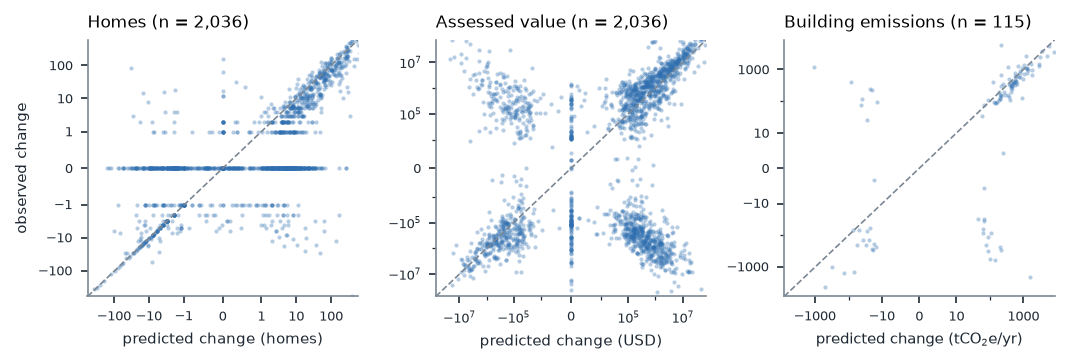
\includegraphics[width=\linewidth]{impact_scatter.png}
\caption{Observed against predicted change on the evaluation lots (symmetric log axes; dashed line: equality).}
\label{fig:s-scatter}
\end{figure}

\paragraph{Direction of change.} Among lots where both changes are non-zero, the predicted change has the observed
sign for 88\% of homes, 60\% of assessed-value changes and 80\% of emissions
changes (Figure~\ref{fig:s-scatter}). The correlation for value is carried by large lots; for a single lot, the
direction of the value change is unreliable.

\paragraph{Jobs.} Job change was tested by 2020 census block (LEHD 2015 and 2023, adjusted for citywide growth), on
blocks with no selection-fold lot: $r = 0.05$ over 837 blocks. The engine has no skill for job
change at this scale, and the Studio marks job change as not validated.

\section{Likelihood, yield and calibration}\label{s:likely}

\paragraph{Outcome.} A lot is developed in $(t_0, t_1]$ if a new building appears on it (Section~\ref{s:leakage}) or
its floor area grows by more than 25\% and 2,000 sq ft. Cross-city definitions follow each source (paper, Section 4).

\paragraph{Manhattan model.} LightGBM (500 trees, learning rate 0.03, 31 leaves, at least 40 lots per leaf, row and
column subsampling 0.8), fitted on all pairs $(a, a+h)$ with $a + h \leq t_0$, on 59 features from the
$t_0$ record: lot and floor area, floors, age, built and permitted FARs, overlay, landmark and historic status, zoning
family, existing use, unused permitted floor area, land share of value, value per square foot, soft-site flag, homes,
neighbour use composition on the parcel graph, and the share of neighbours built in the five years before $t_0$.

\paragraph{Cross-city model.} LightGBM (400 trees, learning rate 0.04, 31 leaves, at least 50 lots per leaf,
subsampling 0.8) on the blocks E, C, Z, P (paper, Section 4), fitted on the first window and tested on the second.

\paragraph{Calibration metrics.} For probabilities $p$ and outcomes $y$ in a test window: reliability in ten
equal-count bins; expected calibration error (bin-weighted absolute gap); observed over predicted events
$\sum y/\sum p$; calibration intercept and slope from a logistic regression of $y$ on $\mathrm{logit}(p)$ (ideal 0 and
1; a slope below 1 means the probabilities are too spread out); and the Brier score against a constant forecast of the
training-period rate, as skill $1 - \mathrm{Brier}/\mathrm{Brier}_\mathrm{prevalence}$.

\paragraph{Recalibration,} using training data only, in two ways: \emph{isotonic}, fitted on the latest training pair
as predicted by a model trained on the earlier pairs (Manhattan, where several pairs exist); and \emph{logistic}
(intercept and slope on $\mathrm{logit}\,p$), fitted on out-of-fold probabilities of the training data from five
spatial folds. Neither uses the test window.

\begin{table}[t]
\centering
\scriptsize
\setlength{\tabcolsep}{2.5pt}
\caption{Calibration of the Manhattan redevelopment model by horizon $h$ (years) and test window: observed over predicted events (O/E), calibration intercept and slope, and Brier skill against the training-period rate; then after temporal isotonic recalibration, and after logistic recalibration on out-of-fold training probabilities.}
\label{tab:s-cal-mn}
\begin{tabular}{llrrrrrrrrrrr}
\toprule
$h$ & Test & Lots & Events & O/E & Int. & Slope & Skill & O/E iso & Skill iso & O/E rec. & Slope rec. & Skill rec. \\
\midrule
1 & 2016--2017 & 42{,}524 & 183 & 0.98 & $-$1.31 & 0.65 & 0.035 & -- & -- & 0.43 & 0.89 & 0.008 \\
1 & 2017--2018 & 42{,}491 & 204 & 1.28 & $-$0.56 & 0.78 & 0.113 & 1.17 & 0.104 & 0.74 & 0.99 & 0.118 \\
1 & 2018--2019 & 42{,}431 & 267 & 1.28 & $-$0.42 & 0.80 & 0.154 & 1.04 & 0.153 & 0.97 & 0.97 & 0.160 \\
1 & 2019--2020 & 42{,}307 & 313 & 1.70 & 0.15 & 0.88 & 0.105 & 1.18 & 0.097 & 1.31 & 1.04 & 0.105 \\
1 & 2020--2021 & 42{,}171 & 14 & 0.07 & $-$2.93 & 0.95 & $-$0.972 & 0.04 & $-$1.762 & 0.06 & 1.05 & $-$0.833 \\
1 & 2021--2022 & 42{,}176 & 128 & 0.91 & $-$0.40 & 0.92 & 0.059 & 12.77 & 0.014 & 0.73 & 1.04 & 0.061 \\
1 & 2022--2023 & 42{,}100 & 73 & 0.56 & $-$1.05 & 0.90 & 0.053 & 0.62 & 0.066 & 0.46 & 1.02 & 0.053 \\
1 & 2023--2024 & 42{,}054 & 139 & 1.16 & $-$0.38 & 0.88 & 0.050 & 2.08 & 0.045 & 0.96 & 0.98 & 0.052 \\
1 & 2024--2025 & 42{,}014 & 126 & 1.06 & $-$0.53 & 0.87 & 0.042 & 0.91 & 0.038 & 0.90 & 0.99 & 0.044 \\
3 & 2018--2021 & 42{,}430 & 570 & 0.81 & $-$1.46 & 0.59 & $-$0.056 & -- & -- & 0.61 & 0.74 & $-$0.032 \\
3 & 2019--2022 & 42{,}307 & 461 & 0.83 & $-$0.82 & 0.80 & 0.079 & 0.77 & 0.012 & 0.65 & 0.95 & 0.082 \\
3 & 2020--2023 & 42{,}171 & 208 & 0.36 & $-$1.49 & 0.88 & $-$0.046 & 0.28 & $-$0.295 & 0.31 & 0.99 & $-$0.037 \\
3 & 2021--2024 & 42{,}175 & 355 & 0.72 & $-$0.60 & 0.93 & 0.075 & 0.92 & 0.044 & 0.63 & 0.94 & 0.064 \\
3 & 2022--2025 & 42{,}099 & 350 & 0.80 & $-$0.67 & 0.87 & 0.054 & 1.04 & 0.029 & 0.73 & 0.83 & 0.035 \\
5 & 2020--2025 & 42{,}170 & 520 & 0.50 & $-$1.25 & 0.83 & 0.046 & -- & -- & 0.40 & 0.97 & 0.033 \\
\bottomrule
\end{tabular}
\end{table}

\begin{table}[t]
\centering
\footnotesize
\setlength{\tabcolsep}{4pt}
\caption{Calibration in each city's test window (existing conditions only, and all blocks): raw, and after logistic recalibration on out-of-fold training-window probabilities.}
\label{tab:s-cal-cities}
\begin{tabular}{llrrrrrrr}
\toprule
City & Blocks & Rate & O/E & Slope & Skill & O/E rec. & Slope rec. & Skill rec. \\
\midrule
Los Angeles & E & 0.33\% & 1.29 & 0.81 & 0.074 & 1.17 & 0.94 & 0.079 \\
 & E+C+Z+P & 0.33\% & 1.59 & 0.80 & 0.058 & 1.24 & 0.97 & 0.070 \\
Dallas & E & 1.33\% & 1.01 & 0.78 & 0.056 & 0.96 & 0.92 & 0.060 \\
 & E+C+Z+P & 1.33\% & 1.18 & 0.88 & 0.129 & 0.97 & 1.03 & 0.132 \\
New York & E & 0.47\% & 1.09 & 0.90 & 0.034 & 1.04 & 0.95 & 0.035 \\
 & E+C+Z & 0.47\% & 1.22 & 0.91 & 0.061 & 1.13 & 1.00 & 0.065 \\
Milwaukee & E & 0.06\% & 0.34 & 0.37 & $-$1.783 & 0.49 & 0.80 & $-$0.230 \\
 & E+C+Z & 0.06\% & 0.42 & 0.21 & $-$2.022 & 0.53 & 0.71 & $-$0.433 \\
Phoenix & E & 0.36\% & 1.12 & 0.57 & 0.038 & 1.10 & 0.76 & 0.048 \\
 & E+C+Z+P & 0.36\% & 1.60 & 0.43 & $-$0.001 & 1.01 & 0.79 & 0.023 \\
San Diego & E & 0.07\% & 0.47 & 0.36 & $-$0.026 & 0.46 & 1.09 & 0.000 \\
 & E+C+Z+P & 0.07\% & 0.78 & 0.55 & $-$0.057 & 0.41 & 1.12 & 0.000 \\
Chicago & E & 0.26\% & 0.80 & 0.82 & 0.000 & 0.76 & 1.03 & 0.005 \\
 & E+C+Z & 0.26\% & 0.86 & 0.87 & $-$0.007 & 0.75 & 1.04 & 0.015 \\
\bottomrule
\end{tabular}
\end{table}

\begin{figure}[h!]
\centering
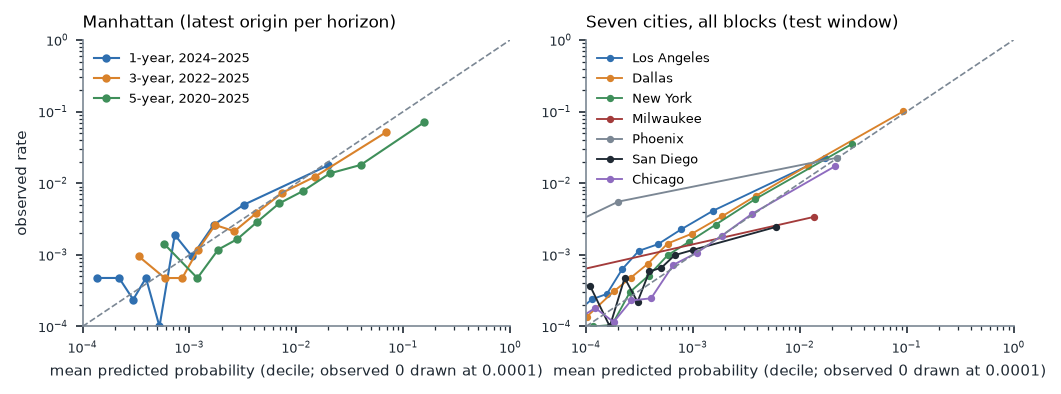
\includegraphics[width=0.85\linewidth]{reliability.png}
\caption{Reliability of redevelopment probabilities (log axes; dashed line: perfect calibration).}
\label{fig:s-reliability}
\end{figure}

\paragraph{From probability to homes.} Three projections are compared with homes built.
\begin{itemize}
\item \textbf{Capacity}: each site built to the permitted floor area at utilisation $\rho$, homes $K_i$.
\item \textbf{Probability $\times$ capacity}: $\sum_i p_i K_i$, where $p_i$ is the probability of redevelopment by the
end of the window. In the rezoning replays the model's horizon $h$ is extended to the $T$ years to 2025 with a
constant hazard, $p_T = 1 - (1-p_h)^{T/h}$.
\item \textbf{Probability $\times$ empirical yield}: redeveloped lots seldom reach capacity. In the cross-city test the
expected yield of a developed lot is the mean homes added by developed lots of the same zoning class (existing class
where zoning is missing) and lot-size bin in the training window (at least 20 lots, else the class, else all lots), so $E[\text{homes}] = \sum_i p_i\,\hat y_i$. In the
rezoning replays it is $\sum_i p_{T,i}\,\bar s\,K_i$, with $\bar s$ the mean share of capacity homes added by soft sites
redeveloped in the training pairs.
\end{itemize}
Probability $\times$ capacity and probability $\times$ yield are expected values of gross homes added (removals are not
subtracted). Their 95\% ranges come from 20,000 draws in which each site is redeveloped independently with its
probability and, for the yield version, takes a share drawn from the training sites. These ranges are conditional on
the model's probabilities: they omit model error and correlation between sites, and are narrower than a full
prediction interval.

\paragraph{Build-out proxy.} In the cross-city test, zoning and plan build-out are not legal capacity (most cities do
not publish maximum FAR as data). Each lot's build-out is the homes per acre that lots whose existing use is in the class its zoning (or
plan) designates reach in the city today (90th percentile among those with homes, at least 30 lots), times its lot
area, minus its homes. It measures what a class's dense lots hold today, not what the rules allow.

\section{Optimizer}\label{s:optimizer}

\paragraph{Objective and constraints.} For a plan $u$ in scope $S$, maximise
\begin{equation}
J(u) = \mathrm{overall}_S(u) - \lambda\,|\{i : u_i \neq u^0_i\}|,\qquad \lambda = 0.0005^\dagger,
\end{equation}
subject to at most $B = \max\{1, \lfloor 0.05^\dagger\, n_\mathrm{eligible}\rfloor\}$ changes. Eligible parcels exclude
landmarks and historic districts, parks, public facilities, transportation and utility lots, and lots without a
known use. Allowed uses on a parcel are those its zoning permits (Section~\ref{s:zoning}); homes may only become
residential or mixed use; built lots may not become open space, parking or vacant land; and converting an existing
building is allowed only if that conversion was observed in Manhattan at that building size or larger (precedent).

\paragraph{First-order gains.} For each parcel and use, the change in $J$ is estimated as
\begin{equation}
g_{iu} = \sum_k a_k\,\Delta x_{iuk} + w_\mathrm{fit}\,[\log P(u\mid\text{context}) - \log P(u^0_i\mid\text{context})] - \lambda,
\end{equation}
where $a_k = 100\,\delta_k\,\omega_k/|b_k|$ for totals and $100\,\delta_k\,\omega_k$ for shares, $\omega_k$ the
indicator's weight in the overall score (pillar weight over the number of indicators in the pillar),
$w_\mathrm{fit} = 0.002^\dagger$, and $\Delta x_{iuk}$ the change in indicator $k$:
\begin{itemize}
\item exact for the additive indicators (homes, jobs, value, green space, runoff, emissions);
\item for access, mix and green cover, the first-order effect on residents within the radius, computed by
convolution on the raster: added open space for residents lacking a park, added floor area for residents in
under-served cells, residents added to under-served cells (dilution), the entropy gradient
$-(\log s_g + H \log 5)/(T\log 5)$ of land-group shares $s_g$ for mix, and the open-space share gradient for green
cover;
\item plus the change in who is counted: a parcel's added residents enter each resident-weighted mean with that
parcel's own value.
\end{itemize}
The gains are exact for additive indicators and first order for the rest, which saturate.

\paragraph{Search.} Iterated best response over 3$^\dagger$ rounds: in round $r$ the
$\lceil(B - \text{changes so far})/(R - r)\rceil$ parcels with the largest positive gain switch to their best use, then
access and gains are recomputed. Because $J$ is the potential function of the game in which each parcel chooses its use,
each round can only improve the estimate. Polishing re-scores exactly the 30$^\dagger$ best moves (add a move,
swap it with the weakest change, or drop a change) for up to two passes. The Studio uses polishing; the candidate plans
for votes do not. The result is the best plan found, not a proven optimum.

\paragraph{Likelihood layer.} When on, candidates are restricted to the fifth of parcels with the highest five-year
probability of redevelopment. Probabilities restrict the candidate set; they do not weight moves.

\paragraph{NSGA-III explorer.} For a selection of parcels, three objectives (the first-order social, economic and
environmental gains) are searched by NSGA-III \citep{deb2014} in pymoo: 45 Das--Dennis reference
directions (eight partitions), population 92, 120 generations, simulated binary crossover
(probability 0.9, $\eta = 15$) and polynomial mutation ($\eta = 20$) with integer rounding, a fixed seed. Every plan
evaluated is archived; the non-dominated plans of the archive are re-scored exactly, plans that another re-scored
plan beats on every pillar are dropped, and at most 24 plans are shown (the best per pillar, then evenly
spaced by total gain).

\paragraph{Test of the explorer.} On Manhattan tax blocks drawn at random, every combination of options was enumerated
(Table~\ref{tab:s-nsga}). On 10 small blocks (64--1{,}024 plans) every plan was also scored exactly;
on 10 medium blocks (24{,}576--327{,}680 plans) the first-order front is known. Quality is the hypervolume of a
front as a share of that of the true front.

\begin{table}[t]
\centering
\footnotesize
\setlength{\tabcolsep}{4pt}
\caption{NSGA-III against the true front: median (minimum) over blocks of the hypervolume share and of the share of true-front plans returned; random search with the same number of evaluations for comparison.}
\label{tab:s-nsga}
\begin{tabular}{lrrrr}
\toprule
Blocks & $n$ & Hypervolume share & Front plans found & Random search \\
\midrule
Small (exact) & 10 & 1.000 (1.000) & 1.000 (0.846) & 1.000 (1.000) \\
Medium (first order) & 10 & 1.000 (0.986) & 0.962 (0.638) & 0.964 (0.944) \\
Medium, re-scored & 10 & 1.000 (0.991) & -- & -- \\
\bottomrule
\end{tabular}
\end{table}

\paragraph{A defect found by this test.} The first version of the first-order model omitted mix and green cover and
the change in who is counted. On small blocks its rank correlation with exact pillar scores fell to
$-$0.35 (environmental), and on one block the explorer's front covered 0.5\% of the exact
front's hypervolume. With the terms above, the rank correlation is at least 0.99 on every pillar.

\section{Decision module}\label{s:decision}

\paragraph{Stakeholders and utilities.} Five agents stand for parties that commonly testify or decide at land-use
hearings: developers (the applicant), residents (community boards and civic associations), environmental advocates,
the city's budget office, and local business associations. Each agent's utility for plan $a$ is
$U_{va} = \sum_k w_{vk}\,\mathrm{score}_k(a)$ with the weights of Table~\ref{tab:s-weights}, so the status quo is worth
zero to everyone. The weights are editable assumptions, not elicited preferences. Each agent holds one seat. One
agent per interest does not represent the variety within it; the residents' referendum below and the sensitivity
tests show how much that matters.

\begin{table}[t]
\centering
\footnotesize
\setlength{\tabcolsep}{3pt}
\caption{Indicator weights of the five stakeholder agents (assumptions; each sums to one).}
\label{tab:s-weights}
\begin{tabular}{lrrrrrrrrrrr}
\toprule
Agent & Homes & Jobs & Value & Park & Services & Facilities & Mix & Green sp. & Runoff & Emissions & Green cov. \\
\midrule
Developer & 0.35 & 0.20 & 0.45 &  &  &  &  &  &  &  &  \\
Residents' association & 0.15 &  &  & 0.25 & 0.20 & 0.20 & 0.10 &  &  &  & 0.10 \\
Environmental advocate &  &  &  &  &  &  &  & 0.30 & 0.20 & 0.30 & 0.20 \\
City budget office & 0.20 & 0.25 & 0.55 &  &  &  &  &  &  &  &  \\
Local business alliance &  & 0.40 &  &  & 0.35 &  & 0.25 &  &  &  &  \\
\bottomrule
\end{tabular}
\end{table}

\paragraph{Candidate plans.} The status quo; each agent's ideal plan (the optimizer with that agent's weights); ten
pairwise compromises (the optimizer with the mean of two agents' weights); a balanced plan (equal pillars); a
consensus plan (only moves that improve every agent's first-order utility); and a parcel-by-parcel ballot (on each
eligible parcel the council ranks the allowed uses by weighted Borda and a change passes with an absolute majority of
seats). All use the same change budget. Identical plans are merged, and every candidate is re-scored exactly.

\paragraph{Rules.} With weighted voters and ties allowed: plurality; Borda; instant runoff; Copeland; Schulze (the
headline rule: Condorcet-consistent, monotone and independent of clones); Kemeny--Young (exact integer program, 10 s
limit); approval (plans better than the status quo); score (utilities rescaled to 0--10 per voter); and majority
judgment (seven grades from utility). Ties are broken by Borda score. Also reported: the Condorcet winner and loser, the
Smith set, whether one voter can change the Schulze result by misreporting, and the Nash bargaining solution with the
status quo as disagreement point.

\paragraph{Residents' referendum.} Today's residents vote by tax block, weighted by population. A block's utility for a
plan is the residents' weights applied to the change in its own access, mix and green cover, plus homes in the study
area; differences below 0.01$^\dagger$ points are ties (just-noticeable difference, an assumption). Future residents
and other areas do not vote.

\paragraph{Robustness and sensitivity.} The winner's Schulze win probability is estimated over 200$^\dagger$
draws in which each indicator's delta is drawn from a triangular distribution over its sensitivity range (one quantile
per indicator, shared by all plans, because a coefficient that is higher than assumed is higher for every plan) and
seats from a Dirichlet distribution centred on the seats (concentration 50$^\dagger$). The sensitivity tests
redraw each agent's weights (Dirichlet, concentration 20), add random feasible plans to the ballot, sweep the
threshold, triple each agent's seats in turn, and draw each block's resident weights independently.

\begin{table}[t]
\centering
\footnotesize
\setlength{\tabcolsep}{4pt}
\caption{Disagreement among the nine rules by candidate set (12 districts): median candidates, median and maximum number of distinct winners, districts where all rules agree and with a Condorcet winner.}
\label{tab:s-vote-sets}
\begin{tabular}{lrrrrr}
\toprule
Candidate set & Candidates & Winners & Max & All agree & Condorcet \\
\midrule
generated & 19 & 4 & 5 & 0 & 7 \\
ideal plans only & 6 & 3 & 4 & 0 & 11 \\
generated + random & 35 & 4 & 5 & 0 & 7 \\
random only & 17 & 2 & 4 & 4 & 11 \\
\bottomrule
\end{tabular}
\par\smallskip
\begin{minipage}{0.95\linewidth}\footnotesize With each block's resident weights drawn independently, the residents' winner is unchanged in a median 100\% of draws.\end{minipage}
\end{table}

\section{Zoning and access as represented}\label{s:zoning}

\begin{itemize}
\item \textbf{Represented}: which of the nine use groups each zoning district permits (simplified rules for New York;
crosswalks of district classes elsewhere), maximum FAR by residential, commercial and community-facility use where the
city publishes it, landmarks and historic districts as protections.
\item \textbf{Not represented}: height and setback limits, lot coverage, parking requirements, inclusionary and other
bonuses, special-district rules, discretionary approvals and building codes. A plan that passes the screen may still
be infeasible.
\item \textbf{Access} uses Euclidean disks on a raster, not walking routes, so barriers such as highways, rail yards
and rivers are ignored and access near them may be overstated.
\end{itemize}

\section{Reproducibility}\label{s:repro}

The code, the result file behind every number, and a manifest of every input (URL, retrieval date, SHA-256) are in the
PlanArena repository; this version is tagged \texttt{v1.1-review}. \texttt{make reproduce} rebuilds the data and every
result from public sources, and \texttt{python -I -m planarena.paper} rebuilds the paper and this supplement from the
result files.

\bibliographystyle{unsrtnat}
\bibliography{../docs/refs}

\end{document}
